\section{Einführung}

	\subsection{Entstehung von Myonen}
	\textit{Myonen} $\mu^{\pm}$ lassen sich im Standardmodell der Teilchenphysik zur zweiten Generation der elektrisch geladenen Leptonen zuordnen. Sie sind mit $m_\mu = 105,658\ \unit{MeV = 206,768\ m_e}$\cite{pdg} die schweren Pendants zum Elektron.\\
	Im folgenden Versuch werden Myonen aus der kosmischen Höhenstrahlung, welche zu 85\% aus hochenergetischen Protonen besteht, untersucht. Bei Zusammenstößen dieser Protonen mit Atomkernen in der Erdatmosphäre entstehen die geladenen $\pi^\pm$-Mesonen Reaktionen niedrigster Ordnung sind:
		\begin{align*}
			&p + p \longrightarrow p + n + \pi^+\\
			&p + n \longrightarrow p + p + \pi-
		\end{align*}
	Diese Mesonen zerfallen nach etwa $2,6\cdot10^{-8}\ \unit{s}$ über die schwache Wechselwirkung. Der mit einem Anteil von 99,988\% dominierende Zerfallskanal endet in einem Myon und einem zugehörigen Neutrino und kann mit folgender Zerfallsgleichung und dem Feynmandiagramm in Abbildung \ref{fig:pionzerfall} beschrieben werden:
		\begin{align*}
			&\pi^+ \longrightarrow \mu^+ + \nu_\mu \text{,}\\
			&\pi^- \longrightarrow \mu^- + \bar{\nu}_\mu \text{.}\\
		\end{align*}
		\begin{figure}[hp]
					\centering
					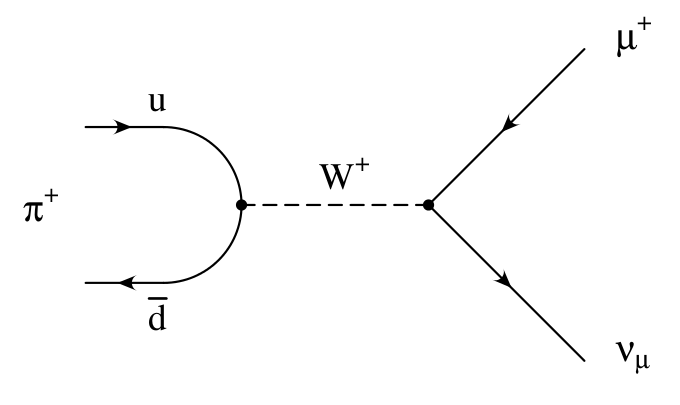
\includegraphics[width = 0.7\linewidth]{pic/pionzerfall.png}
					\caption{Feynman-Diagramm des Antimyonenzerfalls.}
					\label{fig:pionzerfall}
		\end{figure}
		
	\subsection{Zerfall von Myonen}
	Da das Myon ein sehr schweres Teilchen ist, zerfällt es nach einer sehr kurzen Zeit von \cite{PA}:\\
		\begin{equation} \label{eq:lit}
			\tau_\mu = (2,19703 \pm 0,00004)\ \unit{\mu s}
		\end{equation}
	mit nahezu 100\% über den schwachen Zerfall, der mit Hilfe der Reaktionsgleichungen (\ref{eq:mup}) und (\ref{eq:mum}) und zugehörigem Feynmangraph (nur niedrigste Ordnung) in Abbildung \ref{fig:myonzerfall} beschrieben werden kann.\\
	
		\begin{align}
			&\mu^+ \longrightarrow e^+ + \nu_e + \bar{\nu}_\mu 		\label{eq:mup}\\
			&\mu^- \longrightarrow e^- + \bar{\nu}_e + \nu_\mu 		\label{eq:mum}
		\end{align}
		\begin{figure}[hp]
            \centering
            \scalebox{0.5}[0.5]{
  			\input{pic/myonzerfall.pdf_tex}
            }
            \caption{Feynman-Diagramm des Antimyonenzerfalls.}
            \label{fig:myonzerfall}
        \end{figure}
	\ \\
	Auch wenn die in Gleichung (\ref{eq:lit}) angegebene Lebensdauer sehr kurz erscheint, ist der Myonenfluss auf Meereshöhe mit $170\ \unit{Myonen/(m^2s)}$ sehr hoch. Dies lässt sich dadurch erklären, dass die oben angegebene Lebensdauer im Laborsystem der Beobachter auf der Erde angegeben ist. Da sich Myonen mit relativistischen Energien bewegen, besitzen sie in ihrem Ruhesystem eine \textit{zeitdilatierte Lebensdauer}, welche ausreicht, um an die Erdoberfläche zu gelangen. Selbst in der theoretischen Vorhersage der Lebensdauern mit Hilfe von \textit{Übergangsmatrixelementen} $\Gamma_{fi} = 1/\tau_{fi}$ (d.h. bei Übergang von Zustand $\ket{i}$ in $\ket{f}$) treten Terme auf, die nicht lorentzinvariant sind.
	
	\subsection{$\mu^-$-Einfang}
	Im Falle der negativ elektrisch geladenen Myonen $\mu^-$ existiert in Materie allerdings ein weiterer 'Zerfallskanal', der sogenannte $\mu^-$-Einfang, bei dem ein einfallendes Myon im Coulombfeld eines Atoms eingefangen wird bis es den Grundzustand erreicht und anschließend vom Kern absorbiert wird. Dabei findet folgende Kernumwandlung(Abbildung \ref{fig:myoneinfang}) statt:
		\begin{equation*}
			\mu^- + p \longrightarrow  \nu_\mu + n 
		\end{equation*}
		
		\begin{figure}[ht]
			\centering
			\scalebox{1.}[1.]{
			\input{pic/myoneneinfang.pdf_tex}
			}
			\caption{Feynman-Diagramm des Myoneneinfangs.}
			\label{fig:myoneinfang}	
		\end{figure}
	\ \\
	Ist $\Gamma_z = 1/\tau_z$ die Partialbreite  des schwachen Zerfallskanals (\ref{eq:mum}) und $\Gamma_e=1/\tau_e$ die des $\mu^-$-Einfangs, ergibt sich die totale Breite des $\mu^-$-Zerfalls zu:
		\begin{align}
			&\Gamma_{\mu^-} = \Gamma_z + \Gamma_e\\
			&\tau_{\mu^-} = \left(\frac{1}{\tau_z} + \frac{1}{\tau_e}\right)^{-1} < \tau_{\mu^+}  
		\end{align}
	Im Praktikumsversuch werden die Myonen mit einer Kupferplatte eingefangen. Da der $\mu^-$-Einfang dafür sorgt, dass nach etwa $1\ \unit{\mu s}$ alle negativ geladenen Fermionen eingefangen worden, dominieren die $\mu^+$-Zerfälle die Messung. 
	
	\subsection{Messprinzip und Versuchsaufbau}
        \subsubsection{Szintillatoren}
            Szintillatoren sind Körper, die bei Anregung durch Stoßprozesse mit geladenen Teilchen oder Photonen aufgenommene Energie durch Emission von Licht abgeben. Die deponierte Energie lässt sich mittels einer Photodiode oder eines Photomultipliers anhand der Lichtmenge messen. Die Intensität ergibt sich aus der Messung der Szintillationen pro Zeit.
            Es gibt organische und \textbf{anorganische Szintillatoren}. Letztere sind Kristalle, welche mit sogenannten Aktivator-Zentren dotiert sind. Trifft ionisierende Strahlung auf dieses Kristall, erzeugt sie Exzitonen (Elektronen-Loch-Paare), freie Elektronen oder freie Löcher, die sich durch die Struktur bewegen, bis sie ein Aktivator-Zentrum treffen und dieses anregen. Das Aktivator-Zentrum zerfällt infolgedessen unter Emission von Photonen in seinen Grundzustand. 
            \textbf{Organische Szintillatoren} können ebenfalls Kristalle, aber auch Flüssigkeiten oder Polymere sein. Hierbei werden Molekülzustände eines primären Floureszenzstoffes angeregt. Bei deren Zerfall emittieren sie Photonen aus dem UV-Bereich. Da UV-Strahlung in den meisten transparente Materialien jedoch nur kurze Distanzen durchdringt, muss ein weiterer Floureszenzstoff beigefügt werden.
            Dieses Experiment verwendet organische Szintillatoren aus Plaste.
        \subsubsection{Photomultiplier}
            Photoelektronenvervielfacher oder engl. Photomultiplier dienen der Vervielfachung von Elektronen, die durch den äußeren photoelektrischen Effekt aus einer Photokathode herausgelöst wurden. Diese werden durch ein elektrisches Feld beschleunigt und auf Elektroden, die sogenannten Dynoden, gelenkt, um wiederum aus deren Oberfläche mehrere neue Elektronen auszulösen. Dabei löst jedes auftreffende Elektron eine bestimmte Anzahl neue heraus. Die so herausgelösten Elektronen werden ihrerseits zur nächsten Dynode beschleunigt, um jeweils die gleiche Zahl neue Elektronen herauszuschlagen. Die Zahl der herausgelösten Elektronen nimmt damit von einer zur nächsten Stufe exponentiell zu. Um dies zu verwirklichen, muss das Potential mit zunehmendem Weg und wachsender Dynodenstufe immer mehr im positiven Potential liegen. Nach $n$ Dynoden (also $n$ Stufen) können die vervielfachten Elektronen auf eine Anode treffen und über die Masse abfließen, um an einem Widerstand einen Spannungsabfall zu erzeugen, der letztlich das Ausgangssignal der Messung liefert.
            Der Vorgang ist schematisch gut in Abbildung \ref{pm} zu sehen. Mit ihrer Hilfe wird die nach rechts zunehmende Potentialpositivität erreicht. 
            \begin{figure}[htbp]
                \centering 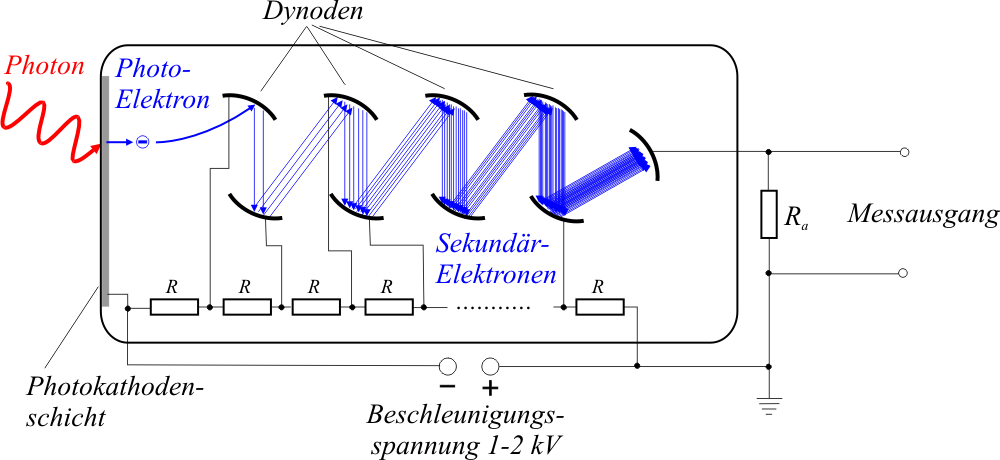
\includegraphics[scale=1]{pic/pm.png}
                \caption{Skizze des Aufbaus eines PM \cite{pm}}
                \label{pm}
            \end{figure}
        \subsubsection{Messprinzip Aufbau 1}
            Wie in Abbildung \ref{prinzip} klar zu erkennen ist, besteht der Aufbau aus PMs, Szintillatoren, Lichtleitern einer Spule und Kupferplatten. Genau genommen besteht der Aufbau aus drei PMs und zwei Kupferplatten der Dicke $1\unit{cm}$. Diese Platten bilden das Target, welches Myonen stoppt, welche in PM3 nicht mehr detektiert werden. Das so ausgelöste Signal ($12\overline{3}$) startet in einem Time-to-Digital-Converter (TDC) eine Zeitmessung, welche entweder durch das Signal $2\cdot\overline 3$ für nach PM2 (oben) oder Signal $\overline 2 \cdot 3$ für nach PM3 (unten) fliegende Positronen gestoppt wird. Durch Start der Zeitmessung wird ein Koinzidenzzeitfenster von $10\unit{\mu s}$ geöffnet, welches zufällige Koinzidenzen stark minimieren soll. Diskriminatoren wandeln die in den Photomultipliern erzeugten Signale in einheitliche Signale mit der Breite von $40\unit{ns}$ um und unterdrücken sämtliche Signale unterhalb von $-200\unit{mV}$.
            Zusätzlich zum Koinzidenzzeitfenster gibt es eine Koinzidenzeinheit, die die benötigten Koinzidenzsignale liefert. Der TDC wandelt seine gemessenen Zeiten in digitale Signale um. Die so gemessenen Ereignisse werden an einen PC übertragen und von diesem über eine Messsoftware ausgelesen und gespeichert. Es existieren für die Auswertung ein oberes und ein unteres Zeitspektrum mit jeweils 256 Kanälen, welche jeweils eine Breite von $1\unit{\mu s}/24,000$ besitzen. \cite{PA} 
            \begin{figure}
                \centering 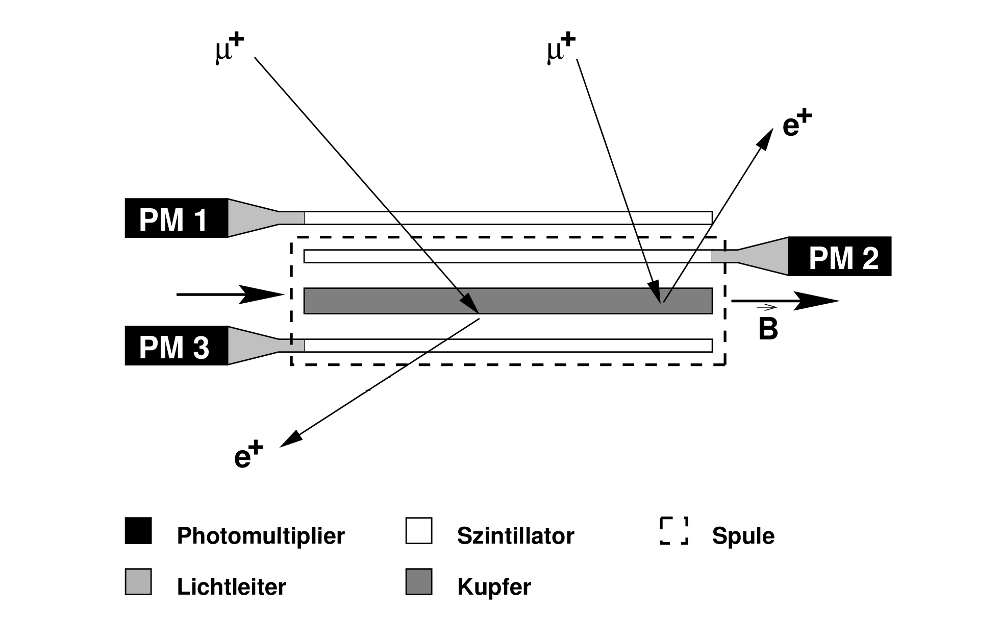
\includegraphics[scale=1.2]{pic/aufbau.png}
                \caption{\cite{pm} Prinzipskizze des Versuchsaufbaus}
                \label{prinzip}
            \end{figure}